\chapter{Opis struktury projektu}
\label{cha:opisStrukturyProjektu}

Projekt zrealizowany został w języku programowania Java z wykorzystaniem technologii JavaFX oraz MySQL. Głównym celem było stworzenie systemu o czytelnej strukturze i dużej elastyczności rozwojowej – łączącego logikę aplikacji z relacyjną bazą danych oraz graficznym interfejsem użytkownika

Do każdego widoku FXML zaimplementowano osobny kontroler, co pozwoliło zachować przejrzystość oraz zgodność paradygmatem MVC. Do realizacji operacji związanych z bazą danych wykorzystano modele odpowiadające poszczególnym tabelom.

Struktura projektu YLO GradeBook została opracowana zgodnie z zasadami dobrych praktyk programistycznych — w sposób ułatwiający jej dalszy rozwój bez konieczności gruntownej przebudowy kodu źródłowego.


% ------------------------------------------------------------------------
\section{Wykorzystane technologie}
W realizacji projektu zastosowano nowoczesne technologie oraz narzędzia, które wspierają tworzenie aplikacji desktopowych o wysokiej wydajności i estetyce interfejsu użytkownika:
\begin{itemize}
    \item Java 23 (OpenJDK) – główny język programowania aplikacji, umożliwiający tworzenie wydajnych aplikacji wieloplatformowych,
    \item JavaFX – biblioteka graficzna umożliwiająca projektowanie interfejsów użytkownika z wykorzystaniem stylizacji i animacji,
    \item FXML – deklaratywny język XML do definiowania struktury widoków graficznych, ułatwiający separację warstwy GUI od logiki aplikacji,
    \item CSS – kaskadowe arkusze stylów, użyte do dostosowania wyglądu interfejsu oraz zapewnienia spójnej estetyki aplikacji,
    \item MySQL + phpMyAdmin – relacyjny system zarządzania bazą danych oraz narzędzie webowe do jej wygodnej administracji,
    \item MySQL Connector/J – sterownik JDBC umożliwiający komunikację aplikacji Java z bazą danych MySQL,
    \item IntelliJ IDEA Community Edition 2024.3.3 – środowisko programistyczne wykorzystywane do implementacji kodu źródłowego,
    \item Scene Builder – aplikacja wspomagająca wizualne projektowanie interfejsów w FXML, znacznie przyspieszająca pracę nad GUI.
\end{itemize}

% ------------------------------------------------------------------------
\newpage
\section{Baza danych}
W celu realizacji projektu \textit{YLO GradeBook} zaprojektowano relacyjną bazę danych o nazwie \textit{gradebook\_data\_base}, stworzoną w systemie MySQL i zarządzaną za pomocą środowiska phpMyAdmin. Jej zadaniem jest przechowywanie danych dotyczących użytkowników, ocen, przedmiotów, terminów, notatek oraz uwag. Struktura bazy została zaprojektowana z uwzględnieniem zasad integralności danych oraz możliwości szybkiego filtrowania i przeszukiwania informacji poprzez odpowiednie relacje pomiędzy encjami. Model został stworzony w sposób umożliwiający łatwą rozbudowę o dodatkowe moduły i funkcjonalności w przyszłości.

\subsection{Struktura encji i relacje}
Baza danych została podzielona na tabele reprezentujące użytkowników, dla roli uczeń powstała tabela zawierająca klasy, do których należą. Utworzono tabele przechowujące dane takie jak terminy, notatki osobiste oraz uwagi, a także tabela z listą przedmiotów szkolnych. Relacje między encjami opierają się na kluczach obcych i pozwalająz achować spójność logiczną oraz integralność danych.

\begin{figure}[H]
    \centering
    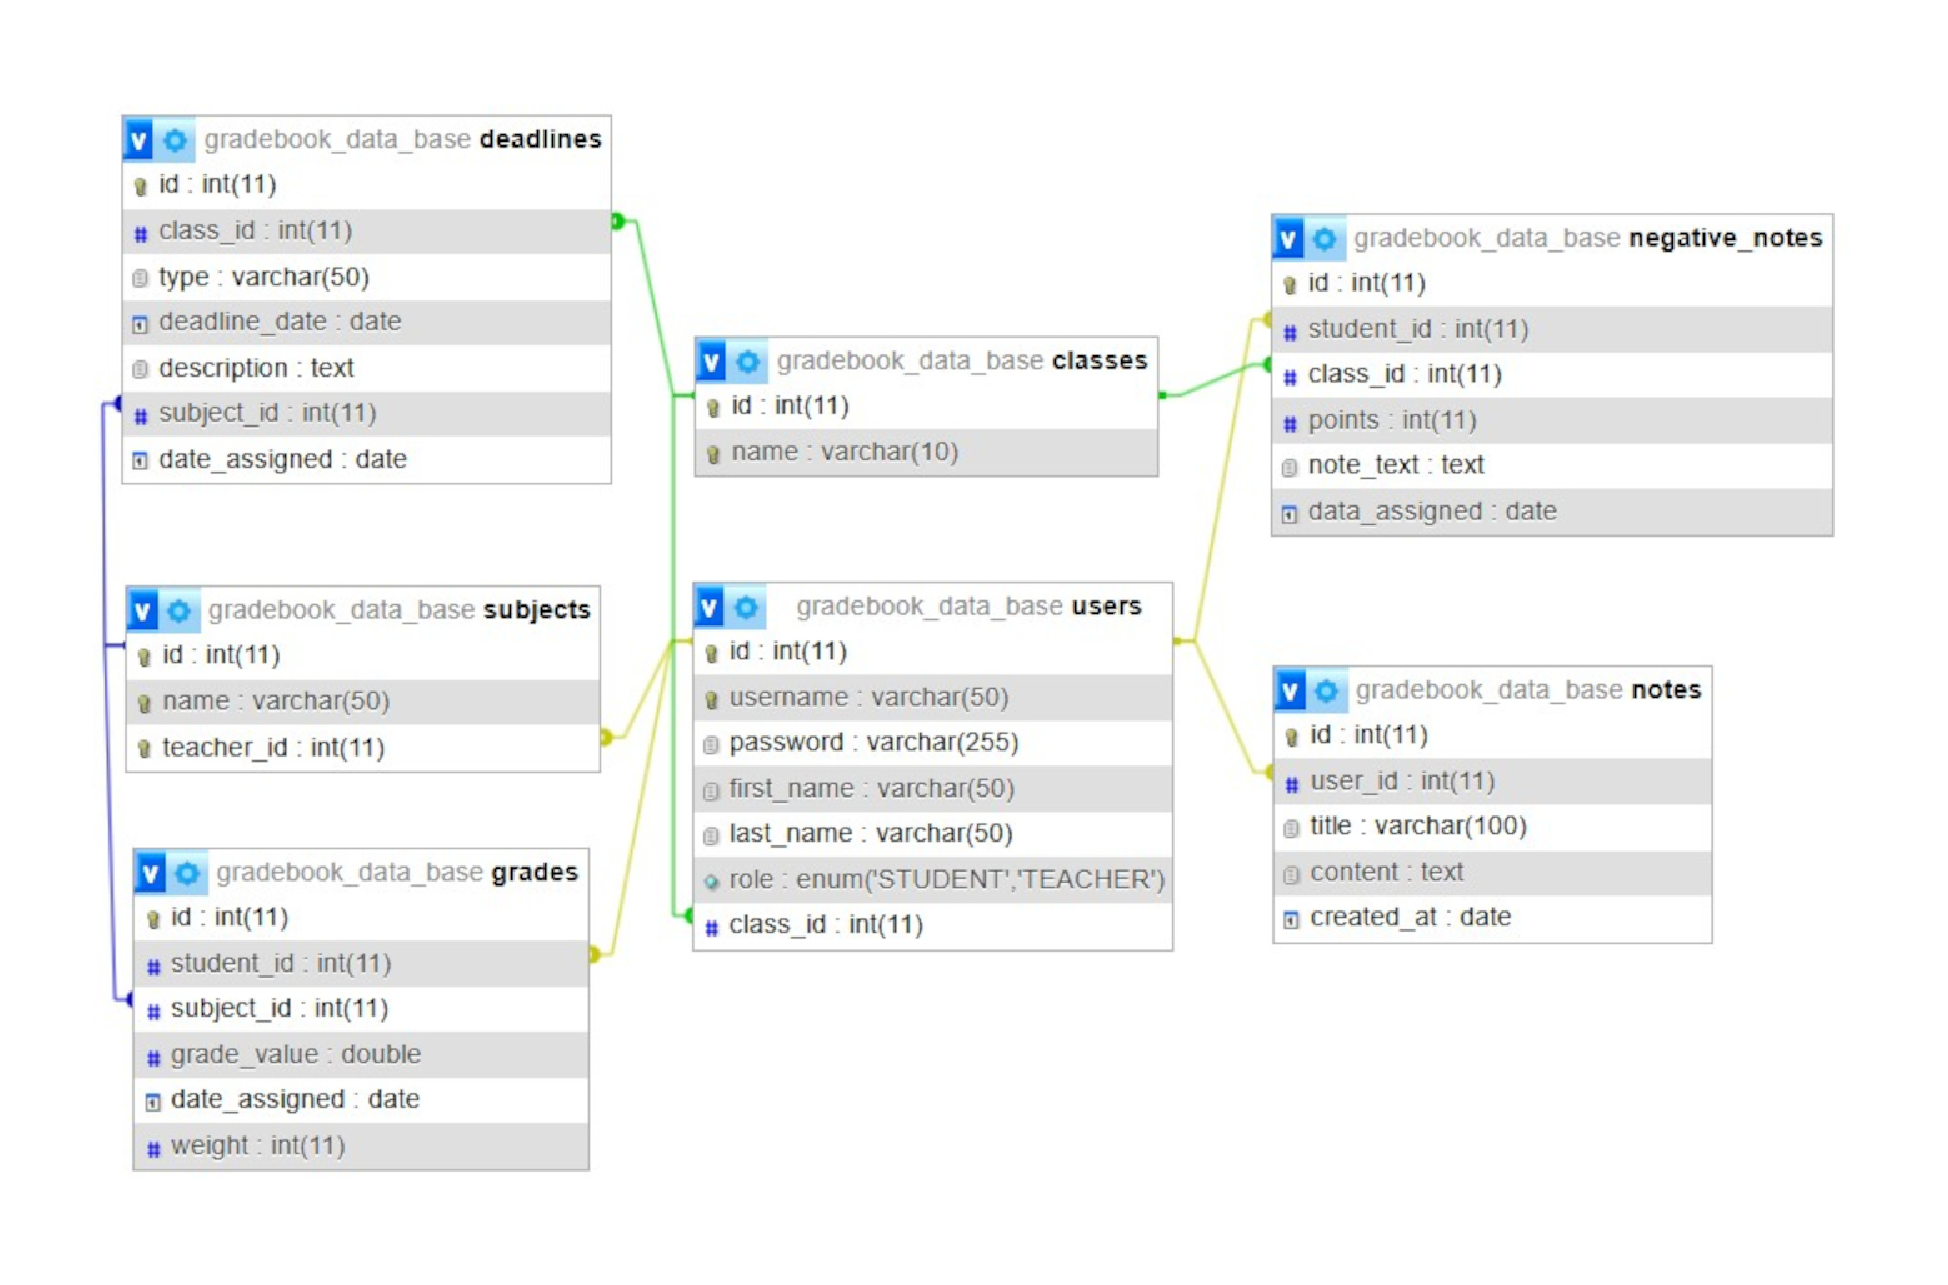
\includegraphics[width=1\textwidth]{figures/fig_0002.eps}
    \caption{Diagram ERD bazy danych \textit{gradebook\_data\_base}}
    \label{fig:erd}
\end{figure}
\newpage
\subsection{Opis tabel}

Struktura bazy danych została zaprojektowana w sposób modularny — każda tabela pełni ściśle określoną funkcję w systemie YLO GradeBook. Tabele powiązane są ze sobą relacjami typu \textit{jeden do wielu} lub \textit{wiele do wielu}, co zapewnia przejrzystość, skalowalność i integralność.

Poniżej przedstawiono opis wszystkich tabel:
\subsubsection*{Tabela \texttt{users}}

Tabela zawiera informacje o wszystkich użytkownikach systemu (uczniach oraz nauczycielach).

\begin{itemize}
    \item \texttt{id} – unikalny identyfikator użytkownika (klucz główny),
    \item \texttt{username}, \texttt{password} – dane logowania,
    \item \texttt{first\_name}, \texttt{last\_name} – dane osobowe,
    \item \texttt{role} – rola użytkownika (np. „student”, „teacher”),
    \item \texttt{class\_id} – odwołanie do tabeli \texttt{classes} (klucz obcy).
\end{itemize}

\subsubsection*{Tabela \texttt{grades}}

Tabela przechowuje oceny przypisywane uczniom.

\begin{itemize}
    \item \texttt{id} – identyfikator oceny (klucz główny),
    \item \texttt{student\_id} – identyfikator ucznia (klucz obcy do \texttt{users}),
    \item \texttt{subject\_id} – przedmiot (klucz obcy do \texttt{subjects}),
    \item \texttt{grade\_value} – wartość oceny (np. 4.5),
    \item \texttt{type} – typ oceny (np. sprawdzian, zadanie),
    \item \texttt{created\_at} – data wystawienia.
\end{itemize}

\subsubsection*{Tabela \texttt{notes}}

Tabela przechowuje notatki osobiste dodawane przez użytkowników systemu.

\begin{itemize}
    \item \texttt{id} – identyfikator notatki (klucz główny),
    \item \texttt{user\_id} – użytkownik, do którego przypisana jest notatka (klucz obcy do \texttt{users}),
    \item \texttt{title} – tytuł notatki,
    \item \texttt{content} – treść notatki,
    \item \texttt{created\_at} – data utworzenia.
\end{itemize}

\subsubsection*{Tabela \texttt{deadlines}}

Tabela przechowuje informacje o nadchodzących terminach.

\begin{itemize}
    \item \texttt{id} – identyfikator terminu (klucz główny),
    \item \texttt{class\_id} – klasa, której dotyczy wydarzenie,
    \item \texttt{subject\_id} – przedmiot związany z terminem,
    \item \texttt{type} – typ wydarzenia (np. sprawdzian, zadanie),
    \item \texttt{date} – data wydarzenia,
    \item \texttt{description} – krótki opis.
\end{itemize}

\subsubsection*{Tabela \texttt{negative\_notes}}

Tabela służy do zapisywania uwag pozytywnych i negatywnych przypisanych uczniom.

\begin{itemize}
    \item \texttt{id} – identyfikator uwagi (klucz główny),
    \item \texttt{student\_id} – uczeń, którego dotyczy uwaga,
    \item \texttt{class\_id} – klasa ucznia,
    \item \texttt{points} – liczba punktów (ujemne/dodatnie),
    \item \texttt{message} – treść uwagi (do 60 znaków),
    \item \texttt{created\_at} – data wystawienia.
\end{itemize}

\subsubsection*{Tabela \texttt{subjects}}

Tabela zawiera przedmioty występujące w systemie.

\begin{itemize}
    \item \texttt{id} – identyfikator przedmiotu (klucz główny),
    \item \texttt{name} – nazwa przedmiotu (np. „matematyka”),
    \item \texttt{teacher\_id} – nauczyciel prowadzący (klucz obcy do \texttt{users}).
\end{itemize}

\subsubsection*{Tabela \texttt{classes}}

Lista klas funkcjonujących w systemie.

\begin{itemize}
    \item \texttt{id} – identyfikator klasy (klucz główny),
    \item \texttt{name} – nazwa klasy (np. „1TIA”),
    \item \texttt{school\_year} – rok szkolny przypisany do klasy.
\end{itemize}


\subsection{Relacje między tabelami}

Relacje pomiędzy tabelami w bazie \textit{gradebook\_data\_base} zostały zaprojektowane w sposób zapewniający pełną integralność danych oraz umożliwiający logiczne powiązanie informacji pomiędzy różnymi obiektami systemu.

\begin{itemize}
     \item Każdy użytkownik (\texttt{users}) przypisany jest do konkretnej klasy (\texttt{classes}), co pozwala na filtrowanie danych względem przynależności uczniów. 
     \item Użytkownicy mogą pełnić rolę ucznia lub nauczyciela, dzięki czemu możliwe jest rozdzielienie funkcjonalność dla obu grup. 
     \item Oceny (\texttt{grades}) są powiązane zarówno z użytkownikiem (uczniem), jak i przedmiotem (\texttt{subjects}), którego dotyczą.      \item Terminy (\texttt{deadlines}) są przypisane do konkretnej klasy i odnoszą się do określonego przedmiotu. \item Notatki (\texttt{notes}) tworzone są indywidualnie przez użytkowników i przypisane tylko do ich kont. 
     \item Uwagi (\texttt{negative\_notes}) są przypisane do ucznia oraz zawierają liczbę punktów (ujemnych lub dodatnich) i treść. 
\end{itemize}

\section*{Podsumowanie}

Struktura bazy danych \textit{gradebook\_data\_base} została zaprojektowana z myślą o przejrzystości, integralności oraz skalowalności danych. Dzięki odpowiednio powiązanym encjom, system pozwala na jednoznaczną identyfikację użytkowników, przypisywanie ocen, notatek, terminów i uwag w kontekście klas i przedmiotów. Zaprojektowana architektura relacyjna nie tylko wspiera bieżącą funkcjonalność aplikacji, ale umożliwia także łatwą rozbudowę systemu w przyszłości — zarówno pod względem danych, jak i logiki aplikacyjnej.

\newpage\newpage
\section{Struktura aplikacji}
\label{sec:strukturaAplikacji}

Aplikacja \textit{YLO GradeBook} została stworzona w języku \textbf{Java} z wykorzystaniem biblioteki \textbf{JavaFX}. Struktura projektu podzielona została na warstwy odpowiadające za logikę, prezentację danych, komunikację z bazą danych oraz wartswę wizualną.

\subsection{Struktura pakietów w projekcie}

Aplikacja \texttt{YLO GradeBook} posiada podział na kilka głównych części: 

\begin{itemize}
    \item \texttt{pakiet główny} – zawiera wszystkie klasy aplikacji odpowiedzialne za:
    \begin{itemize}
        \item logikę kontrolerów powiązanych z plikami \texttt{.fxml},
        \item klasę startową \texttt{Main.java},
        \item połączenie z bazą danych (\texttt{DataBaseConnection.java}),
        \item klasy pomocnicze
    \end{itemize}

    \item \texttt{models} – pakiet zawierający klasy odwzorowujące encje z bazy danych. Każdy model reprezentuje jedną tabelę.
    \item \texttt{resources} – pakiet zawierający pliki wykorzystywane w warstwie prezentacji, takie jak:
    \begin{itemize}
        \item pliki FXML opisujące strukturę widoków graficznych,
        \item style CSS odpowiadające za wygląd interfejsu,
        \item czcionki i ikony wykorzystywane w interfejsie użytkownika.
    \end{itemize}
\end{itemize}

Chociaż klasy w pakiecie głównym nie zostały podzielone na pod-pakiety ze względu na funkcjonalność, zastosowano odpowiednie nazewnictwo, które jasno określa ich przeznaczenie. Dzięki temu struktura pozostaje spójna i zrozumiała.

\subsection{Opis zaimplementowanych klas}

Diagram klas (rys. \ref{fig:diagramUML}) przedstawia strukturę głównych komponentów systemu, ich wzajemne relacje dziedziczenia oraz implementację. 
\subsubsection*{Main.java}
Klasa startowa aplikacji. Zawiera metodę \texttt{start()} z JavaFX i ładuje widok logowania (\texttt{LoginWindow.fxml}). Odpowiada za inicjalizację sceny głównej i ustawienie tytułu aplikacji.

\subsubsection*{DataBaseConnection.java}
Klasa służy do połączenia z bazą danych \texttt{MySQL}. Wykorzystuje sterownik JDBC oraz dane logowania zapisane w kodzie.

\subsubsection*{MainWindow.java}
Klasa pełniąca zadanie kontrolera dla głównego kontenera (\texttt{MainWindow.fxml}) do ładowania poszczególnych widoków.

\subsubsection*{ViewLoadingManager.java}
Klasa pomocnicza pełniąca funkcję menadżera ładowania widoków. Każda metoda przyjmuje nazwę pliku \texttt{.fxml} i zastępuje bieżący widok w kontenerze \texttt{MainWindow.fxml}.

\subsubsection*{Session.java}
Klasa pomocnicza przechowująca informacje o zalogowanym użytkowniku, dzięki czemu w trakcie trwania sesji aplikacji mamy dostęp do jego danych.

\subsubsection*{SessionController.java}
Abstrakcyjna klasa bazowa zawierająca metody do wyświetlania komunikatów systemowych (błędy, ostrzeżenia, informacje). Umożliwia klasom pochodnym stosowanie jednolitego mechanizmu komunikacji z użytkownikiem, eliminując powielanie kodu.

\subsubsection*{AuthenticationInterface.java}
W strutkturze skorzystano z możliwości implementacji interfejsu, który wymusza na klasach go implementujących zdefiniowanie odpowiednich metod. Metody, które implementuje umożliwiają pokazywanie hasła podczas logowania lub resetowania hasła oraz pozwalające na włączenie możliwości przemieszczanie się tabulatorem po interfejsie użytkownika.

\subsubsection*{LoginWindow.java}
Kontroler powiązany z widokiem \texttt{LoginWindow.fxml}. Odpowiada za logowanie użytkownika i zapis jego danych w klasie \texttt{Session}. Implementuje interfejs \texttt{AuthenticationInterface}, co umożliwia m.in. obsługę pokazywania hasła oraz przełączanie fokusu tabulatorem. Udostępnia również metodę otwierającą widok resetowania hasła.

\subsubsection*{PasswordReset.java}
Kontroler przypisany do widoku \texttt{PasswordReset.fxml}. Pozwala na aktualizację hasła użytkownika po podaniu poprawnych danych. Również implementuje interfejs \texttt{AuthenticationInterface} i definiuje odpowiednie metody zgodne z tym widokiem.

\subsubsection*{StudentWindow.java}
Kontroler odpowiadający za widok \texttt{StudentWindow.fxml}. Odpowiada za obsługę graficznego interfejsu ucznia, który zawiera panele z ocenami, terminami, uwagami oraz notatkami osobistymi. Klasa odpowiada m.in. za:
\begin{itemize}
    \item ładowanie i aktualizowanie danych ucznia (oceny, średnia, uwagi, terminy),
    \item filtrowanie wpisów dodanych w ciągu ostatnich 7 dni,
    \item obsługę notatek użytkownika (dodawanie i usuwanie),
    \item przełączanie widoków i obsługę przycisków w panelu bocznym,
    \item dostęp do widoków danych osobowych oraz zmiany hasła.
\end{itemize}
\newpage
\subsubsection*{TeacherWindow.java}
Kontroler widoku \texttt{TeacherWindow.fxml}, pełniący funkcję głównego panelu nauczyciela. Klasa umożliwia:
\begin{itemize}
    \item przegląd uczniów przypisanych do wybranej klasy,
    \item przegląd i analizę ocen z podziałem na przedmioty i uczniów,
    \item dodawanie ocen, terminów, uwag oraz notatek osobistych,
    \item zarządzanie widokiem danych osobowych i zmiany hasła,
    \item przełączanie sekcji aplikacji za pomocą panelu nawigacyjnego.
\end{itemize}

\subsubsection*{PopUpWindow.java}
Klasa pomocnicza obsługująca otwieranie widoków typu \textit{popup} w osobnych oknach. Umożliwia ładowanie plików \texttt{.fxml} zawierających formularze, np. do dodawania ocen, terminów, notatek czy uwag. Zapewnia spójny i modularny sposób wyświetlania dodatkowych interfejsów użytkownika bez zakłócania głównego widoku.

\subsection{Modele}
\label{sec:moduly}

W strukturze systemu zastosowano modele odpowiadające tabelom bazy danych, co umożliwia odwzorowanie danych w postaci obiektów Java. Każda klasa modelowa zawiera zestaw atrybutów reprezentujących kolumny w tabeli oraz odpowiednie metody dostępowe (gettery i settery).

\begin{itemize}
    \item \texttt{Classes.java} – reprezentuje klasę uczniowską; zawiera m.in. nazwę klasy.
    \item \texttt{Deadlines.java} – odwzorowuje terminy wydarzeń przypisanych do klas i przedmiotów, takich jak sprawdziany czy kartkówki.
    \item \texttt{Grade.java} – odpowiada za pojedynczą ocenę ucznia.
    \item \texttt{NegativeNote.java} – przechowuje informacje o punktowych uwagach przypisanych do uczniów, zarówno pozytywnych, jak i negatywnych.
    \item \texttt{Note.java} – model notatki utworzonej przez użytkownika, zawierający tytuł i treść.
    \item \texttt{StudentGrade.java} – pomocniczy model wykorzystywany do wyświetlania ocen z przypisanym przedmiotem i obliczoną średnią ocen.
    \item \texttt{Subject.java} – reprezentuje przedmiot szkolny.
    \item \texttt{Users.java} – ogólny model użytkownika systemu (ucznia lub nauczyciela), przechowujący dane logowania, imię, nazwisko i rolę.
\end{itemize}

\section*{}
\begin{figure}[H]
    \centering
    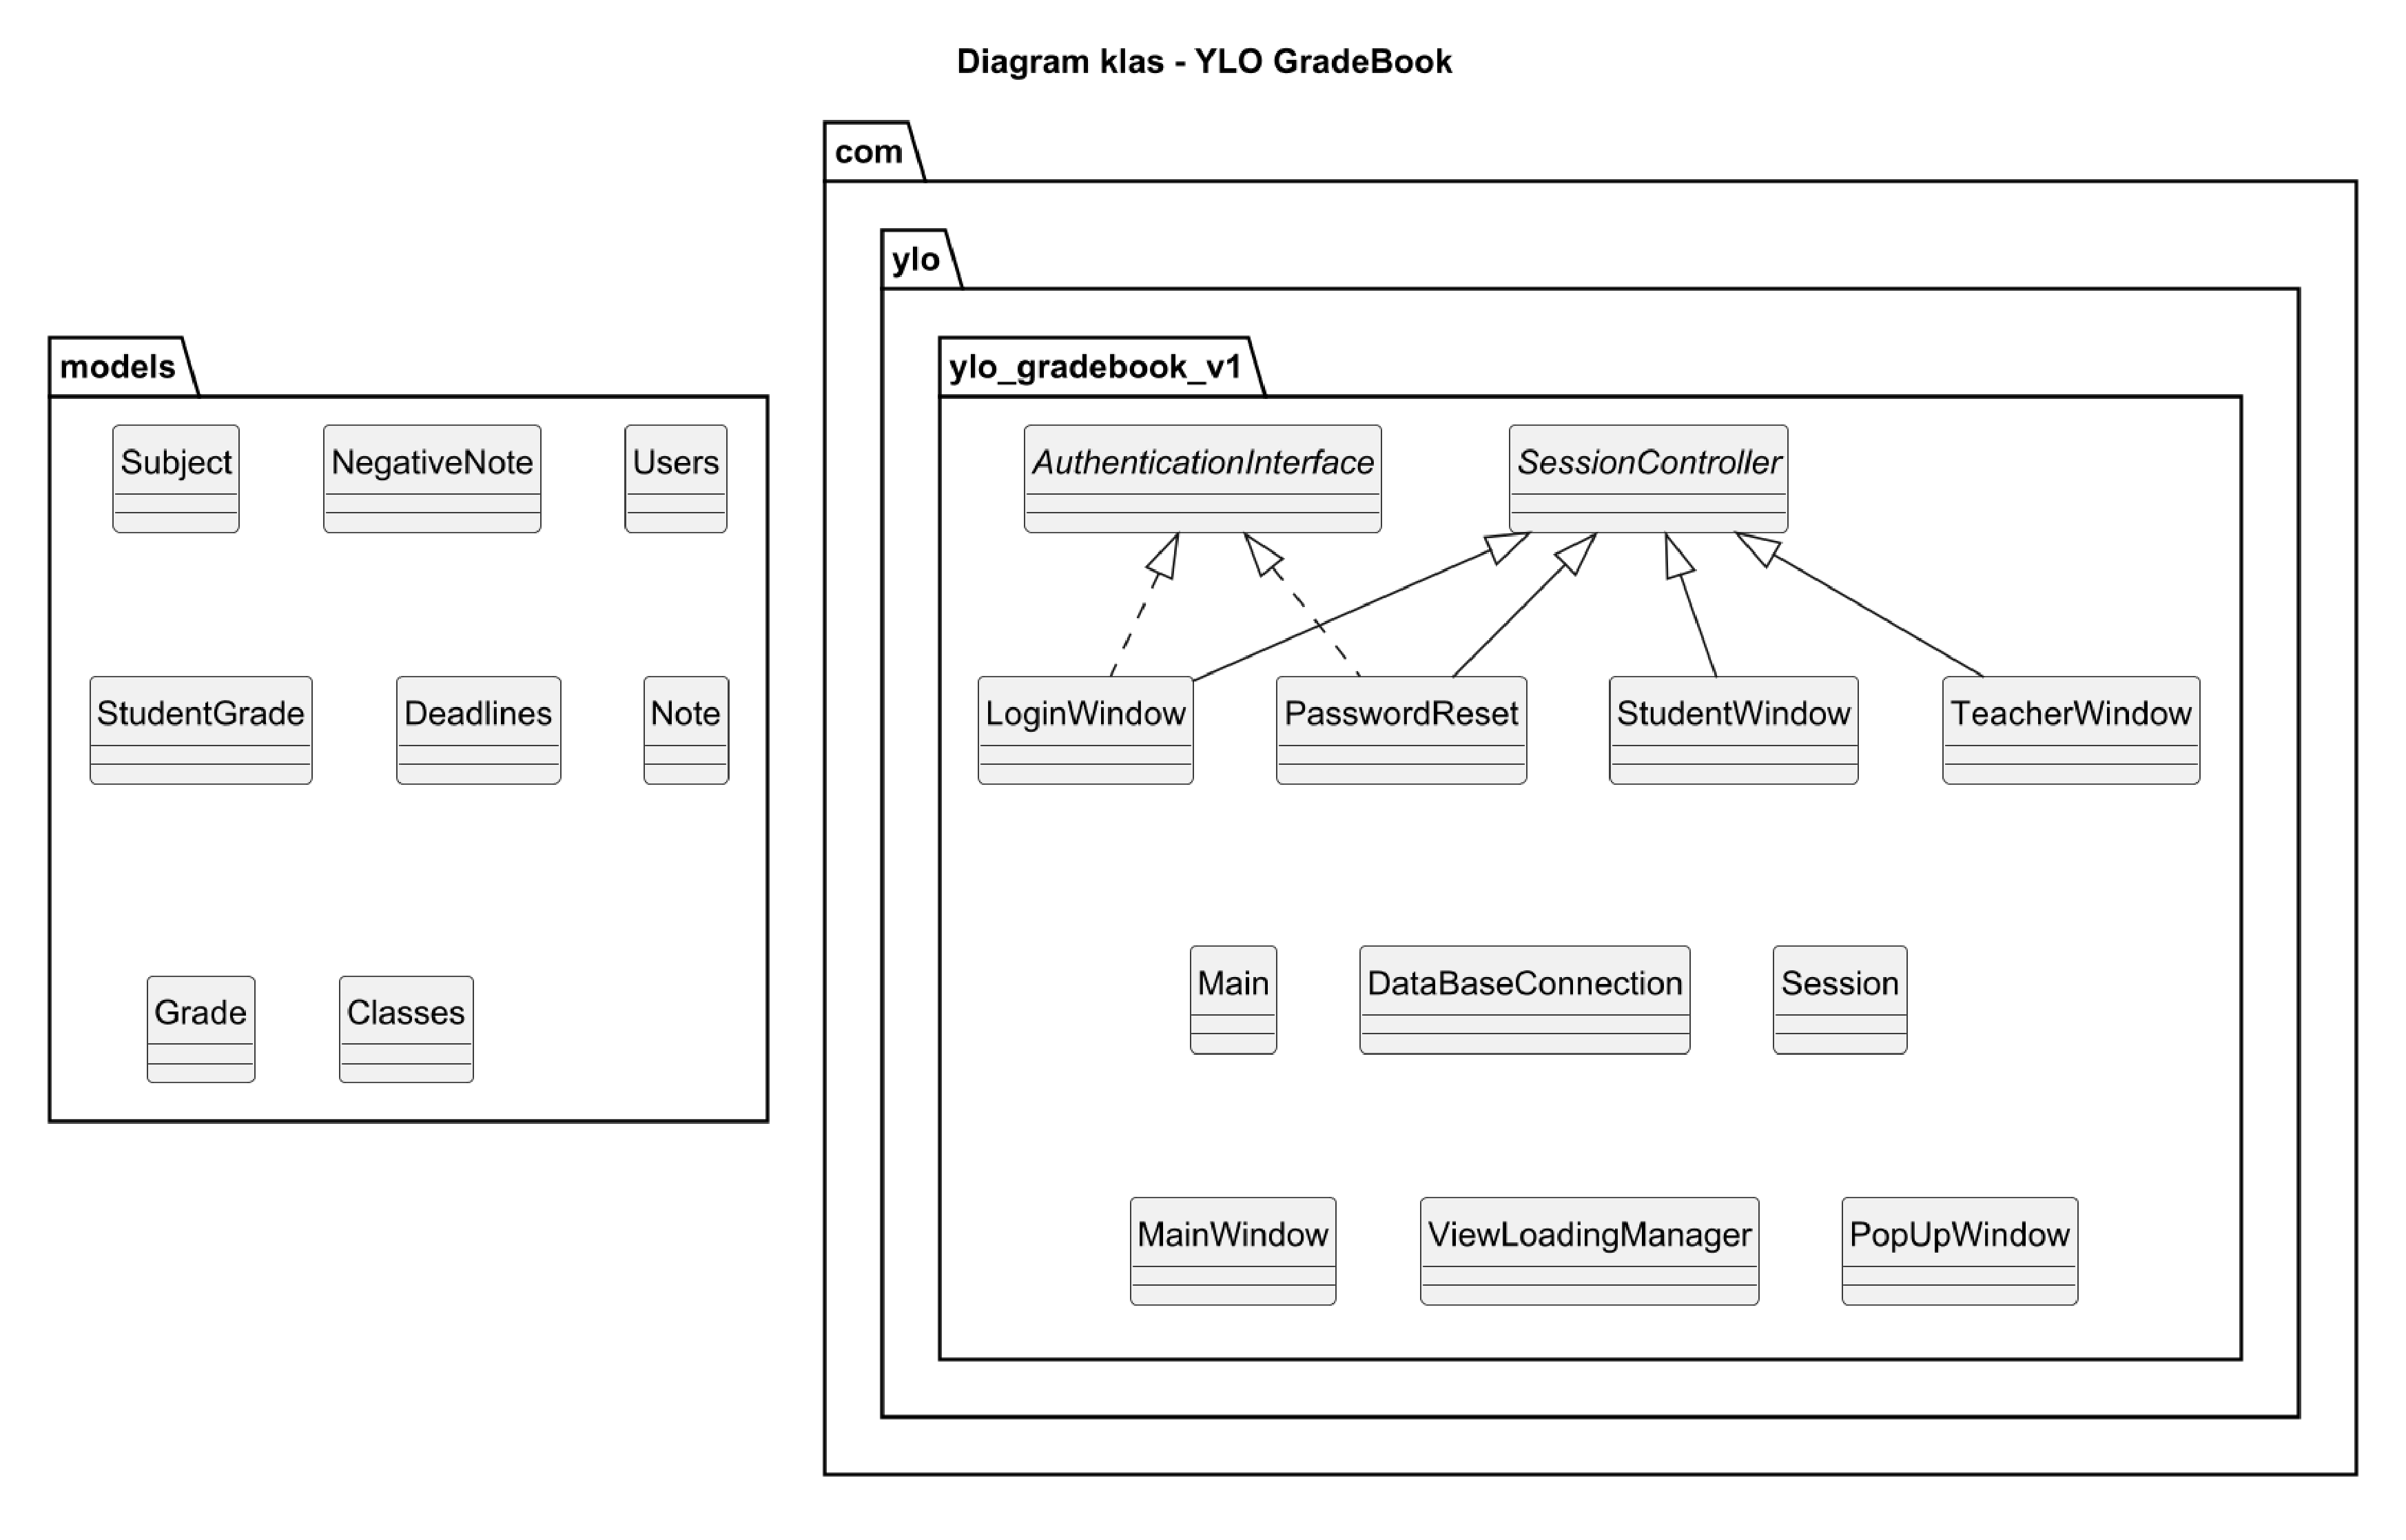
\includegraphics[width=1\textwidth]{figures/fig_0003.eps}
    \caption{Diagram klas systemu YLO GradeBook}
    \label{fig:diagramUML}
\end{figure}



\subsection{Widoki graficzne (FXML)}
\label{sec:widokiFXML}

Interfejs użytkownika aplikacji \texttt{YLO GradeBook} został zaprojektowany z użyciem technologii \textbf{FXML}, co umożliwia oddzielenie warstwy wizualnej od logiki aplikacji. Każdy plik FXML odpowiada konkretnemu widokowi i powiązany jest ze swoim kontrolerem w języku \texttt{Java}.

\begin{itemize}
    \item \texttt{MainWindow.fxml} – główny kontener aplikacji, do którego ładowane są pozostałe widoki (ucznia lub nauczyciela). Stanowi miejsce dynamicznie zmieniających się widoków.
    \item \texttt{LoginWindow.fxml} – widok logowania. Zawiera pola do wpisania loginu i hasła, przycisk logowania oraz odnośnik do resetowania hasła. Umożliwia użytkownikowi dostęp do systemu.
    \item \texttt{PasswordReset.fxml} – formularz zmiany hasła. Zawiera pola do wprowadzenia loginu, nowego hasła i jego potwierdzenia.
    \item \texttt{PopUpWindow.fxml} – szablon wykorzystywany do wyświetlania popupów, np. do dodawania ocen, terminów, notatek czy uwag. Umożliwia ładowanie okien pomocniczych bez zakłócania pracy głównej aplikacji.
    \item \texttt{StudentWindow.fxml} – główny widok ucznia. Zawiera pasek nawigacyjny, umożliwiający przełączanie się pomiędzy wieloma zakładkami. Zawiera rozbudowaną strukturę, która realizuje wszystkie funkcje udostępnione dla roli ucznia.
    \item \texttt{TeacherWindow.fxml} – główny widok nauczyciela. Udostępnia pełną funkcjonalność do zarządzania danymi. Podobnie jak widok ucznia posiada panel nawigacyjny do przełączania się między zakładkami.
\end{itemize}

\subsection{Pozostałe zasoby}
Folder \texttt{resources} zawiera nie tylko pliki FXML odpowiadające widokom graficznym, ale także zasoby wizualne, które wspierają spójny i nowoczesny wygląd aplikacji. W jego strukturze znajdują się:
\begin{itemize}
    \item \texttt{styles/} – pliki CSS definiujące styl graficzny aplikacji. Wpływają one na kolory, marginesy, zaokrąglenia przycisków i ogólną estetykę interfejsu użytkownika.
    \item \texttt{icons/} – zestaw ikon w formacie \texttt{.png}, wykorzystywany w przyciskach, paskach nawigacyjnych i oknach popup. Ułatwiają szybką identyfikację funkcji.
    \item \texttt{fonts/} – pliki czcionek używane w interfejsie. Ich dołączenie zapewnia spójność typograficzną.
\end{itemize}

Zestaw ikon użytych w interfejsie graficznym pochodzi ze strony \texttt{www.freepik.com}. Ikony zostały pobrane w ramach licencji wymagającej przypisania autorstwa i były modyfikowane graficznie na potrzeby projektu.  

Zastosowanie zasobów oddzielonych od logiki aplikacji zwiększa przejrzystość projektu i ułatwia jego stylowanie bez ingerencji w kod źródłowy.
